% !TEX root = ../maturaarbeit.tex
\chapter{Diskussion}\label{chap:diskussion}
Diskussion der Messdaten...

\section{Eine Figur}\label{sec:eine figur}
In \fref{fig:matlabfigur} kann man schöne Farben erkennen. Im Gegensatz dazu sehen die Formeln aus \fref{sec:ueber einstein} ein bisschen blass aus. Man erkennt auch eine gewisse Grösse von \LaTeX, Referenzen zu setzen.
\begin{figure}[ht]
	\centering
	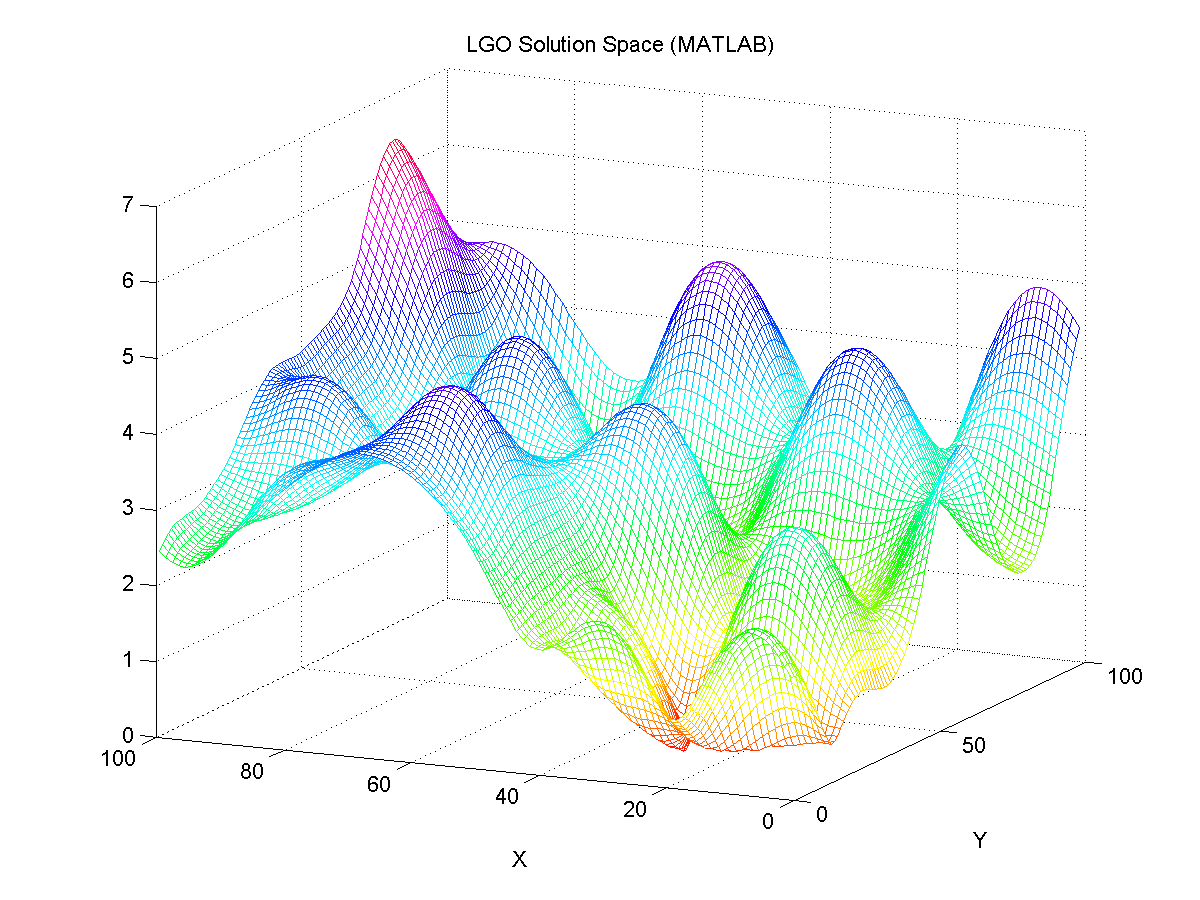
\includegraphics[scale=0.3]{figures/matlabgraph}
	\caption[MATLAB Plot]{Ein Plot aus dem Internet \cite{Plot}, der mit MATLAB erstellt wurde.}
	\label{fig:matlabfigur}
\end{figure}

\newpage